\documentclass{proc}

\title{Exploring neural network optimisations using MNIST}
\author{Stefanos Stefanou(020363)}
\usepackage[margin=0.3in]{geometry}
\usepackage{amsmath}
\usepackage{tikz}
\usepackage{textgreek}
\usepackage{listings}
\usetikzlibrary{positioning}
\tikzset{%
	every neuron/.style={
		circle,
		draw,
		minimum size=0.1cm
	},
	neuron missing/.style={
		draw=none, 
		scale=1,
		text height=0.1cm,
		execute at begin node=\color{black}$\vdots$
	},
}
\begin{document}
	\maketitle
	\section{Abstract}
	Multilayer Neural Networks trained using back-propagation algorithm are the best example of a successful
	Gradient-Based Learning technique.In this report we will going to explore an application of an MN N , handwritten 
	patterns recognition.We will tune our MN N application in order to be able to handle efficiently the dozens(or even hundreds) of neurons and hidden layers, using basic linear algebra rules
	\section{Introduction}

	\subsection{Structure}
	we have used an OOP approach to synthesize our solution, with 2 basic classes, NeuralNetwork and PerceptronMultilayer.NeuralNetwork class is a wrapper over multiple PerceptronMultilayer objects.it handles and supervises their learning by injecting them the proper data during learning
	\subsection{The Algorithm}
	In order to perform our experiments in a reasonable amount of time, a new approach was needed. so we we-wrote our Multilayer Neural Network engine , using matrix multiplications. this reduced the learning time significantly
	\subsubsection{Calculating a layer}
	let the following sigmoid-activated MNN
	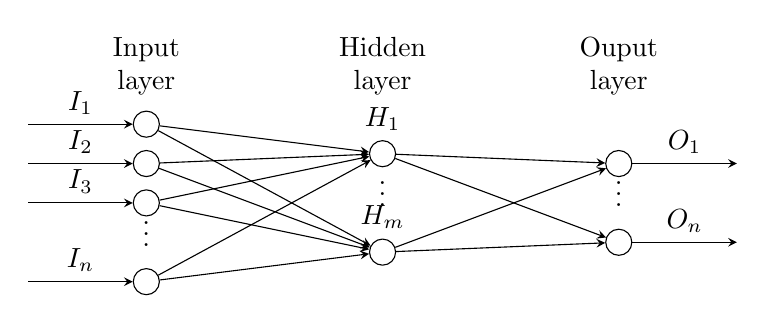
\begin{tikzpicture}[x=1.5cm, y=0.5cm, >=stealth]
	
	\foreach \m/\l [count=\y] in {1,2,3,missing,4}
	\node [every neuron/.try, neuron \m/.try] (input-\m) at (0,2.5-\y) {};
	
	\foreach \m [count=\y] in {1,missing,2}
	\node [every neuron/.try, neuron \m/.try ] (hidden-\m) at (2,2-\y*1.25) {};
	
	\foreach \m [count=\y] in {1,missing,2}
	\node [every neuron/.try, neuron \m/.try ] (output-\m) at (4,1.5-\y) {};
	
	\foreach \l [count=\i] in {1,2,3,n}
	\draw [<-] (input-\i) -- ++(-1,0)
	node [above, midway] {$I_\l$};
	
	\foreach \l [count=\i] in {1,m}
	\node [above] at (hidden-\i.north) {$H_\l$};
	
	\foreach \l [count=\i] in {1,n}
	\draw [->] (output-\i) -- ++(1,0)
	node [above, midway] {$O_\l$};
	
	\foreach \i in {1,...,4}
	\foreach \j in {1,...,2}
	\draw [->] (input-\i) -- (hidden-\j);
	
	\foreach \i in {1,...,2}
	\foreach \j in {1,...,2}
	\draw [->] (hidden-\i) -- (output-\j);
	
	\foreach \l [count=\x from 0] in {Input, Hidden, Ouput}
	\node [align=center, above] at (\x*2,2) {\l \\ layer};
	
	\end{tikzpicture}
	The calculation of a single layer can be done by multiplying the weights of the current layer with the transposed matrix inputs
	\[
	\begin{bmatrix}
	w_{11} & w_{12} & w_{13} & \dots  & w_{1m} \\
	w_{21} & w_{22} & w_{23} & \dots  & w_{2m} \\
	\vdots & \vdots & \vdots & \ddots & \vdots \\
	w_{m1} & w_{m2} & w_{m3} & \dots  & w_{nm}
	\end{bmatrix}
	\begin{bmatrix}
	x_{1}\\
	x_{2}\\
	\vdots\\
	x_{m}
	\end{bmatrix}
	=
	\begin{bmatrix}
	$$\sum_{i=1}^{n} x_iw_{1i}$$ \\
	$$\sum_{i=1}^{n} x_iw_{2i}$$ \\
	\vdots \\
	$$\sum_{i=1}^{n} x_iw_{mi}$$
	\end{bmatrix}
	\]
	the following python code implements this algorithm
		\begin{lstlisting}[language=Python]
def run(self, prev_layer_out):
  sum=np.dot(self.weights,prev_layer_out.T)
  result=sigmoid(sum)
  return result.T
	\end{lstlisting}
	 \subsubsection{Training the output layer}
	 let the M targets, O be the outputs(after the activation function is applied) and I be the inputs of the output layer
	 \[
	 T=
	 \begin{bmatrix}
	 t_{1}\\
	 t_{2}\\
	 \vdots\\
	 t_{m}
	 \end{bmatrix}, 	 
	 O=
	 \begin{bmatrix}
	 o_{1}\\
	 o_{2}\\
	 \vdots\\
	 o_{m}
	 \end{bmatrix},
	 I=
	 \begin{bmatrix}
	 i_{1}\\
	 i_{2}\\
	 \vdots\\
	 \vdots\\
	 i_{n}
	 \end{bmatrix}    
	 \]
	 then, by defining ${\odot}$ to be Hadamard multiplication, the matrix of deltas in the output layer will be..
	 \[
	 \Delta=
	 (T-O)\odot(1-O)\odot O=
	 \begin{bmatrix}
	 (t_{1} - o_{1})(1-o_{1})o_{1}\\
	 (t_{2} - o_{2})(1-o_{2})o_{2}\\
	  \vdots\\
	 (t_{m} - o_{m})(1-o_{m})o_{m}
	  \end{bmatrix} 
	 =
	 \begin{bmatrix}
	 \delta_1\\
	 \delta_2\\
	 \vdots\\
	 \delta_m
	 \end{bmatrix} 
	 \]
	let \texteta{} be the MNN's learning rate, then the correction matrix will be
	\[
	C=I(\Delta\eta)^T= 
	\begin{bmatrix}
		\delta_1i_1\eta & \delta_1i_2\eta & \delta_1i_3\eta & \dots  & \delta_1i_m\eta \\
		\delta_2i_1\eta & \delta_2i_2\eta & \delta_2i_3\eta & \dots  &  \delta_2i_m\eta \\
		\vdots & \vdots & \vdots & \ddots & \vdots \\
		\delta_ni_1\eta & \delta_ni_2\eta & \delta_ni_3\eta & \dots  & \delta_ni_m\eta
	\end{bmatrix}
	\]
	The python code implementing this algorithm is given below
	\begin{lstlisting}[language=Python]
def term_learn(self, i, o, t):
  t=t.reshape(1,self.output_len)
  o=t.reshape(1, self.output_len)
  Delta=np.array((t-o)*(1.0-o)*o)
  correction=i*Delta.T
  self.weights+=correction
	\end{lstlisting}
%	then, we apply the correction to the output layers weights
%	\[
%	\begin{bmatrix}
%	w_{11}+\delta_1i_1\eta & w_{12}+\delta_1i_2\eta & w_{13}+\delta_1i_3\eta & \dots  & w_{1m}+\delta_1i_m\eta \\
%	w_{21}+\delta_2i_1\eta & w_{22}+\delta_2i_2\eta & w_{23}+\delta_2i_3\eta & \dots  & w_{2m}+\delta_2i_m\eta \\
%	\vdots & \vdots & \vdots & \ddots & \vdots \\
%	w_{n1}+\delta_ni_1\eta & w_{n2}+\delta_ni_2\eta & w_{n3}+\delta_ni_3\eta & \dots  & w_{nm}+\delta_ni_m\eta
%	\end{bmatrix}
%	\]
	\subsubsection{Training the hidden layer}
	let the $\Delta_r$, W\textsubscript{r} be the deltas and the weight matrices  of r'th layer respectively
	\[
	\Delta_r=
	\begin{bmatrix}
	\delta_1\\
	\delta_2\\
	\vdots\\
	\delta_m
	\end{bmatrix} 	 
	W_r=
	\begin{bmatrix}
	w_{11} & w_{12} & w_{13} & \dots  & w_{1m} \\
	w_{21} & w_{22} & w_{23} & \dots  & w_{2m} \\
	\vdots & \vdots & \vdots & \ddots & \vdots \\
	w_{m1} & w_{m2} & w_{m3} & \dots  & w_{nm}
	\end{bmatrix} 
	\]
	Next, we define ${E_r(i)}$ to be the error of i'th neuron at r'th layer
	\[ E_r(i)=\sum_{j=1}^{n} \delta_{r+1}(j)*w_{r+1}(j,i)  \]
	It can be easily seen that...
	\[
	W_{r+1}^T\Delta_{r+1}=
	\begin{bmatrix}
	\sum_{j=1}^{n} \delta_{r+1}(j)*w_{r+1}(j,1)\\
	\sum_{j=1}^{n} \delta_{r+1}(j)*w_{r+1}(j,2)\\
	\vdots\\
	\sum_{j=1}^{n} \delta_{r+1}(j)*w_{r+1}(j,m)
	\end{bmatrix} 
	=
	\begin{bmatrix}
	 E_r(1)\\
	 E_r(2)\\
	\vdots\\
	 E_r(m)
	\end{bmatrix} 
	\]
	
	so ,our delta matrix will become
	\[
	\Delta_r=
	W_{r+1}^T\Delta_{r+1}\odot(1-O)\odot O=
	\begin{bmatrix}
	E_r(1)(1-o_{1})o_{1}\\
	E_r(2)(1-o_{2})o_{2}\\
	\vdots\\
	E_r(m)(1-o_{m})o_{m}
	\end{bmatrix} 
	=
	\begin{bmatrix}
	\delta_1\\
	\delta_2\\
	\vdots\\
	\delta_m
	\end{bmatrix} 
	\]
	The rest of the procedure is identical to section 2.2.2, the following code implements this algorithm
	\begin{lstlisting}[language=Python]
def mid_learn(self,i,next_layer,o):
 Wr_p_1=next_layer.weights
 Dr_p_1=next_layer.Delta
 self.Delta=Wr_p_1.T*Dr_p_1
 self.Delta=self.Delta*(1-o)*o
 self.Delta=i*self.Delta.T*self.learning_rate
 self.weights+=self.Delta
	\end{lstlisting}
	\subsection{Technologies}
	In our application we have used a number of new technologies in order to cope with the natural complexity of the given task.We completely rewrite our Multilayer Neural Network engine using python3.6, in order to have available the following, as a result
	\subsubsection{numpy}
	numpy is a mathematics library for python, it offers fast matrix multiplication and dot product implementations, vital for our approach in MN N's
	\subsubsection{matplotlib}
	matplotlib is a ploting library for python, we used to visualise our data and results
	\subsubsection{pickle}
	pickle is a fast csv loader for python , it is vital to our applications performance
		
	\section{User Application}
	The MNIST Database(Modified National Institute of Standards and Technology)consists of 60.000 train and 10.000 test examples of handwritten digits.It is a standardised test in machine learning and is used as common ground for researches to compare their results.
	Our dataset is contained in 2 csv files, training and testing data.Every line of these files consists of an 28x28 image, given as exactly 784 numbers , between 0(white pixel) and 255(black pixel). An additional number at the beginning of each line is for the numbers label
	\subsection{Preprocessing}
	\subsubsection{Normalised Labels}
	We need to perform "Binarization" to MNIST's labels, this can be done using one-hot representation. Each line of every csv file starts with a number ${k[0<=k<=9]}$ and will be converted as follows
	
	\begin{tabular}{ccccc}
			1&                      2&                      \dots&                      9&                      \\
			(100000000)&                      (01000000)&                     \dots&                       (000000001)&                      \\
			\multicolumn{1}{l}{} & \multicolumn{1}{l}{} & \multicolumn{1}{l}{} & \multicolumn{1}{l}{} & \multicolumn{1}{l}{}
	\end{tabular}
	\subsubsection{Normalised Pixels}
	We will convert the default grayscale interval to a range [0,1], by dividing each pixel value with 255. This becomes huge problem though, because it allows for zero inputs, something that if occur can prevent the neuron from learning, so we need to eradicate zeros as inputs, by applying the following function in every pixel.
	\[
		f(x)=\frac{x*0.99}{255}+0.01
	\]
	\subsection{Initialization}
	As it turns out, initialization is a very important factor in our application success, we cant choose random initialization weights. Weight matrices should be chosen randomly but not arbitrary.By choosing a random normal distribution we have broken possible symmetries, which may affect negatively the learning process.
	
	let ${n}$ be the number of inputs in our network, our initialization procedure draws random numbers from a truncated normal distribution as follows
	
	\[
		{\displaystyle X\sim{\frac {1}{\sigma }}\,{\frac {\phi ({\frac {x-\mu }{\sigma }})}{\Phi ({\frac {b-\mu }{\sigma }})-\Phi ({\frac {a-\mu }{\sigma }})}}},
	\]
	\[	a=-\frac{1}{\sqrt(n)},
		b=\frac{1}{\sqrt(n)},
		\mu=0,
		\sigma=1
	\] 
	\subsection{Fragmentation of data}
	MNIST Database has already provide us with a basic fragmentation of our data. 60.000 train and 10.000 test elements, but extensive care has been given in order minimise the uncertainty factor and not over-train our MNN[1].
	
	As reference [1] finds, "the fraction of patterns reserved for the
	validation set should be inversely proportional to the square root of the number of free adjustable
	parameters"
	\begin{tabular}{ccc}
		train&                    60000&                     	\\ 
		test&                     4000&                  		\\
		validation&               6000							
	\end{tabular}

	\subsection{Structure of MNN}
	In order to ensure the optimal output, multiple experiments will be performed, using various hidden layer configurations, as a common ground though, the following rules will be followed in every experiment.
	
	
	\begin{itemize}
		\item every pixel will become a free adjustable parameter, in the input layer
		\item as handwritten digits is a purely categorical variable, the output layer will always consists of 10 Neurons, one for each digit category
	\end{itemize}
	
	 
	\begin{tikzpicture}[x=1.5cm, y=0.5cm, >=stealth]
	
	\foreach \m/\l [count=\y] in {1,2,3,missing,n}
	\node [every neuron/.try, neuron \m/.try] (input-\m) at (0,2.5-\y) {};
	
	\foreach \m [count=\y] in {1,missing,2}
	\node [every neuron/.try, neuron \m/.try ] (hidden-\m) at (2,2-\y*1.25) {};
	
	\foreach \m [count=\y] in {1,missing,2}
	\node [every neuron/.try, neuron \m/.try ] (output-\m) at (4,1.5-\y) {};
	
	\foreach \l [count=\i] in {1,2,3,\textsuperscript{784}}
	\draw [<-] (input-\i) -- ++(-1,0)
	node [above, midway] {$I_\l$};
	
	\foreach \l [count=\i] in {1,m}
	\node [above] at (hidden-\i.north) {$H_\l$};
	
	\foreach \l [count=\i] in {1,\textsuperscript{10}}
	\draw [->] (output-\i) -- ++(1,0)
	node [above, midway] {$O_\l$};
	
	\foreach \i in {1,...,4}
	\foreach \j in {1,...,2}
	\draw [->] (input-\i) -- (hidden-\j);
	
	\foreach \i in {1,...,2}
	\foreach \j in {1,...,2}
	\draw [->] (hidden-\i) -- (output-\j);
	
	\foreach \l [count=\x from 0] in {Input, Hidden, Ouput}
	\node [align=center, above] at (\x*2,2) {\l \\ layer};
	
	\end{tikzpicture}
	\section{Results}
	"Lorem ipsum dolor sit amet, consectetur adipiscing elit, sed do eiusmod tempor incididunt ut labore et dolore magna aliqua. Ut enim ad minim veniam, quis nostrud exercitation ullamco laboris nisi ut aliquip ex ea commodo consequat. Duis aute irure dolor in reprehenderit in voluptate velit esse cillum dolore eu fugiat nulla pariatur. Excepteur sint occaecat cupidatat non proident, sunt in culpa qui officia deserunt mollit anim id est laborum."
	"Lorem ipsum dolor sit amet, consectetur adipiscing elit, sed do eiusmod tempor incididunt ut labore et dolore magna aliqua. Ut enim ad minim veniam, quis nostrud exercitation ullamco laboris nisi ut aliquip ex ea commodo consequat. Duis aute irure dolor in reprehenderit in voluptate velit esse cillum dolore eu fugiat nulla pariatur. Excepteur sint occaecat cupidatat non proident, sunt in culpa qui officia deserunt mollit anim id est laborum."
	\section{Discussion}
	"Lorem ipsum dolor sit amet, consectetur adipiscing elit, sed do eiusmod tempor incididunt ut labore et dolore magna aliqua. Ut enim ad minim veniam, quis nostrud exercitation ullamco laboris nisi ut aliquip ex ea commodo consequat. Duis aute irure dolor in reprehenderit in voluptate velit esse cillum dolore eu fugiat nulla pariatur. Excepteur sint occaecat cupidatat non proident, sunt in culpa qui officia deserunt mollit anim id est laborum."
	"Lorem ipsum dolor sit amet, consectetur adipiscing elit, sed do eiusmod tempor incididunt ut labore et dolore magna aliqua. Ut enim ad minim veniam, quis nostrud exercitation ullamco laboris nisi ut aliquip ex ea commodo consequat. Duis aute irure dolor in reprehenderit in voluptate velit esse cillum dolore eu fugiat nulla pariatur. Excepteur sint occaecat cupidatat non proident, sunt in culpa qui officia deserunt mollit anim id est laborum."
	\section{Conclusion}
	"Lorem ipsum dolor sit amet, consectetur adipiscing elit, sed do eiusmod tempor incididunt ut labore et dolore magna aliqua. Ut enim ad minim veniam, quis nostrud exercitation ullamco laboris nisi ut aliquip ex ea commodo consequat. Duis aute irure dolor in reprehenderit in voluptate velit esse cillum dolore eu fugiat nulla pariatur. Excepteur sint occaecat cupidatat non proident, sunt in culpa qui officia deserunt mollit anim id est laborum."
	"Lorem ipsum dolor sit amet, consectetur adipiscing elit, sed do eiusmod tempor incididunt ut labore et dolore magna aliqua. Ut enim ad minim veniam, quis nostrud exercitation ullamco laboris nisi ut aliquip ex ea commodo consequat. Duis aute irure dolor in reprehenderit in voluptate velit esse cillum dolore eu fugiat nulla pariatur. Excepteur sint occaecat cupidatat non proident, sunt in culpa qui officia deserunt mollit anim id est laborum."
	\section{References}
	"Lorem ipsum dolor sit amet, consectetur adipiscing elit, sed do eiusmod tempor incididunt ut labore et dolore magna aliqua. Ut enim ad minim veniam, quis nostrud exercitation ullamco laboris nisi ut aliquip ex ea commodo consequat. Duis aute irure dolor in reprehenderit in voluptate velit esse cillum dolore eu fugiat nulla pariatur. Excepteur sint occaecat cupidatat non proident, sunt in culpa qui officia deserunt mollit anim id est laborum."
	"Lorem ipsum dolor sit amet, consectetur adipiscing elit, sed do eiusmod tempor incididunt ut labore et dolore magna aliqua. Ut enim ad minim veniam, quis nostrud exercitation ullamco laboris nisi ut aliquip ex ea commodo consequat. Duis aute irure dolor in reprehenderit in voluptate velit esse cillum dolore eu fugiat nulla pariatur. Excepteur sint occaecat cupidatat non proident, sunt in culpa qui officia deserunt mollit anim id est laborum."
\end{document}